\documentclass[12pt, titlepage]{article}

\usepackage{amsmath, mathtools}

\usepackage[round]{natbib}
\usepackage{amsfonts}
\usepackage{amssymb}
\usepackage{graphicx}
\usepackage{colortbl}
\usepackage{xr}
\usepackage{hyperref}
\usepackage{longtable}
\usepackage{xfrac}
\usepackage{tabularx}
\usepackage{float}
\usepackage{siunitx}
\usepackage{booktabs}
\usepackage{multirow}
\usepackage[section]{placeins}
\usepackage{caption}
\usepackage{fullpage}
\usepackage[letterpaper, portrait, margin=1in]{geometry}
\usepackage{helvet}
\usepackage{afterpage}
\usepackage{titlepic}
\usepackage[dvipsnames]{xcolor}

\usepackage{titlesec}
\titleformat{\section}{\large\bfseries\color{RedOrange}}{\rlap{\color{black}\rule[-0.3cm]{\linewidth}{1cm}} {\textcolor{RedOrange}{\thesection}}}{1em}{}

\renewcommand{\familydefault}{\sfdefault}

\hypersetup{
bookmarks=true,     % show bookmarks bar?
colorlinks=true,       % false: boxed links; true: colored links
linkcolor=red,          % color of internal links (change box color with linkbordercolor)
citecolor=blue,      % color of links to bibliography
filecolor=magenta,  % color of file links
urlcolor=cyan          % color of external links
}

\usepackage{array}

\externaldocument{../../SRS/SRS}

%% Comments

\usepackage{color}

\newif\ifcomments\commentstrue %displays comments
%\newif\ifcomments\commentsfalse %so that comments do not display

\ifcomments
\newcommand{\authornote}[3]{\textcolor{#1}{[#3 ---#2]}}
\newcommand{\todo}[1]{\textcolor{red}{[TODO: #1]}}
\else
\newcommand{\authornote}[3]{}
\newcommand{\todo}[1]{}
\fi

\newcommand{\wss}[1]{\authornote{blue}{SS}{#1}} 
\newcommand{\plt}[1]{\authornote{magenta}{TPLT}{#1}} %For explanation of the template
\newcommand{\an}[1]{\authornote{cyan}{Author}{#1}}

%% Common Parts

\newcommand{\progname}{ProgName} % PUT YOUR PROGRAM NAME HERE
\newcommand{\authname}{Team \#, Team Name
\\ Student 1 name and macid
\\ Student 2 name and macid
\\ Student 3 name and macid
\\ Student 4 name and macid} % AUTHOR NAMES                  

\usepackage{hyperref}
    \hypersetup{colorlinks=true, linkcolor=blue, citecolor=blue, filecolor=blue,
                urlcolor=blue, unicode=false}
    \urlstyle{same}
                                


\begin{document}

\title{\textbf{Module Interface Specification for \progname{}} \\ \vspace{2cm} 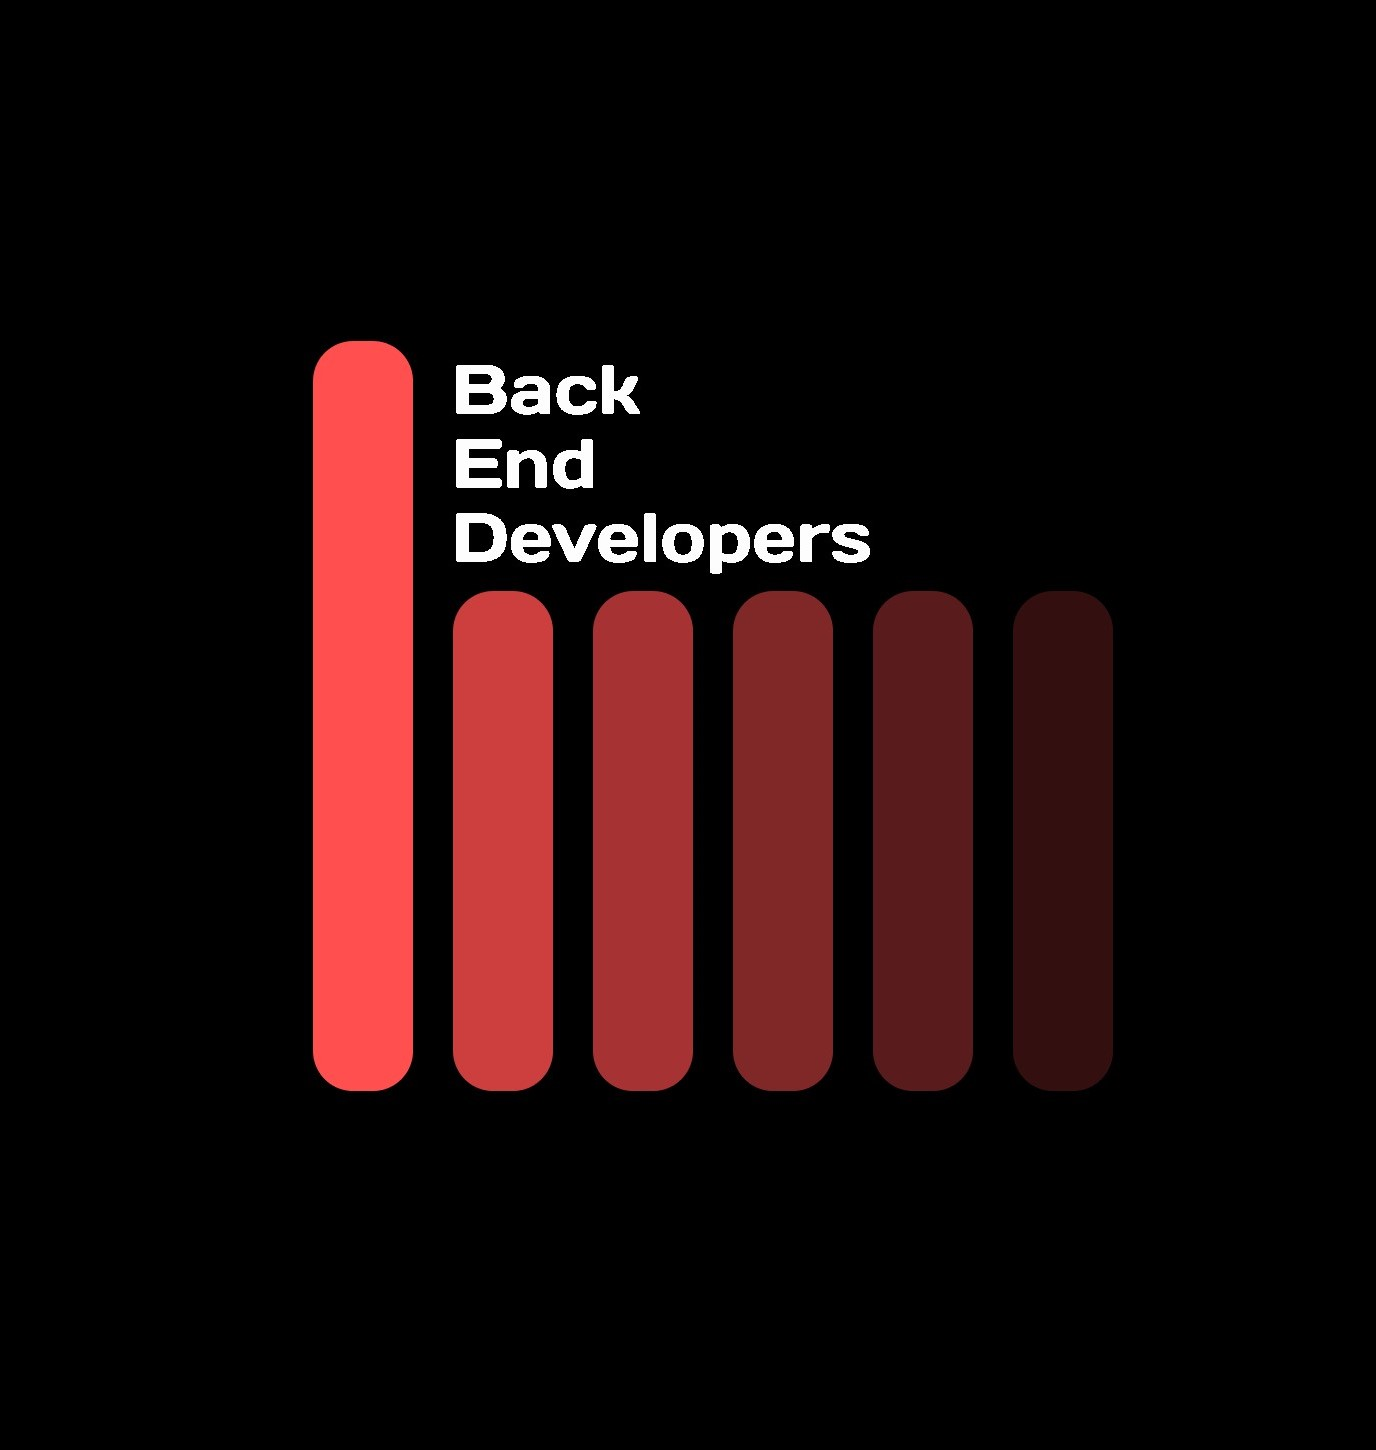
\includegraphics[width=0.5\textwidth]{../../logo.jpg}}
\author{\authname}

\date{\today}
 \pagecolor{black}\afterpage{\nopagecolor}
\color{white}\maketitle

\color{black}
\pagenumbering{roman}

\section{Revision History}

\begin{tabularx}{\textwidth}{p{3cm}p{2cm}X}
\toprule {\bf Date} & {\bf Version} & {\bf Notes}\\
\midrule
2023-01-18 & 1.0 & Initial documentation\\
2023-03-15 & 2.0 & Minor improvements and proof reading for revision 1\\
2023-04-03 & 2.1 & Incorporated TA feedback\\
2023-04-03 & 2.2 & Included logo and added style to the document\\
\bottomrule
\end{tabularx}

~\newpage

\section{Symbols, Abbreviations and Acronyms}

Please refer to the System Requirements Specifications document at \href{https://github.com/zakerl/Capstone_Project/blob/desDoc_Labeeb/docs/SRS/SRS.pdf}{this link} for relevant symbols, abbreviations.\\

\newpage

\tableofcontents

\newpage

\pagenumbering{arabic}

\section{Introduction}

The following document details the Module Interface Specifications for the EMAnator; the system currently being developed by the Back End Developers designed to aid in Ecological Momentary Assessment research. This document describes the various relevant details of interfacing with each module. These details include  module descriptions, the uses of each module, the syntax of each module, and the semantics associated with each module.\\

Complementary documents include the System Requirement Specifications and the Module Guide. The Back End Developers highly recommend a thorough read-through of each document prior to a reading of this document to attain the prerequisite knowledge necessary to fully understand this MIS. The System Requirements Specifications can be found at \href{https://github.com/zakerl/Capstone_Project/blob/main/docs/SRS/SRS.tex}{this link}, and the Module Guide can be found at \href{https://github.com/zakerl/Capstone_Project/blob/main/docs/Design/SoftArchitecture/MG.pdf}{this link}.

\section{Notation}

The structure of the MIS for modules comes from \citet{HoffmanAndStrooper1995},
with the addition that template modules have been adapted from
\cite{GhezziEtAl2003}.  The mathematical notation comes from Chapter 3 of
\citet{HoffmanAndStrooper1995}.  For instance, the symbol := is used for a
multiple assignment statement and conditional rules follow the form $(c_1
\Rightarrow r_1 | c_2 \Rightarrow r_2 | ... | c_n \Rightarrow r_n )$.

The following table summarizes the primitive data types used by \progname. 

\begin{center}
\renewcommand{\arraystretch}{1.2}
\noindent 
\begin{tabular}{l l p{7.5cm}} 
\toprule 
\textbf{Data Type} & \textbf{Notation} & \textbf{Description}\\ 
\midrule
Character & char & A single symbol or digit\\
Integer & $\mathbb{Z}$ & A number without a fractional component in (-$\infty$, $\infty$) \\
Natural number & $\mathbb{N}$ & A number without a fractional component in [1, $\infty$) \\
Real & $\mathbb{R}$ & Any number in (-$\infty$, $\infty$)\\
\bottomrule
\end{tabular} 
\end{center}

\noindent
The specification of \progname \ uses some derived data types: sequences, strings, and
tuples. Sequences are lists filled with elements of the same data type. Strings
are sequences of characters. Tuples contain a list of values, potentially of
different types. In addition, \progname \ uses functions, which
are defined by the data types of their inputs and outputs. Local functions are
described by giving their type signature followed by their specification.

\section{Module Decomposition}

The following table is taken directly from the Module Guide document for this project.
\begin{table}[h!]
  \centering
  \begin{tabular}{|p{0.3\textwidth} | p{0.3\textwidth} |p{0.3\textwidth}  |}
    \toprule
    \textbf{Level 1}        & \textbf{Level 2}        &\textbf{Level 3} \\
    \midrule

    \multirow{9}{0.3\textwidth} {Hardware-Hiding Module}              & Battery Management       & Battery\\
\cline{2-3}
					                                                          &  \multirow{2}{0.3\textwidth}{Data Storage}        & microSD     \\
																		&			&Database\\
\cline{2-3}
					                                                          & \multirow{3}{0.3\textwidth}{Sensor Array}         & Sensor Reading    \\
																		&			& Sensor Data Processing \\
																		&			& Sensor Prompt Validity \\ 
\cline{2-3}
												  & \multirow{2}{0.3\textwidth}{Physical Design} & Watch Straps \\
																		&			& Watch Case \\

    \midrule

    \multirow{3}{0.3\textwidth}{Behaviour-Hiding Module}  & Display System         & Display Screen  \\
\cline{2-3}
			                                                          & Prompt Generation       & Prompt Generation \\
\cline{2-3}
			                                                          & Real Time Clock      & RTC   \\


    \midrule

    \multirow{4}{0.3\textwidth}{Software Decision Module} &  \multirow{2}{0.3\textwidth}{Parameter Selection}& Create New User\\
																		&			& Configuration \\
\cline{2-3}
                                                          & \multirow{2}{0.3\textwidth}{Data Processing}       & Graph  \\
											&			& Data Display \\

    \bottomrule
  \end{tabular}
  \caption{Module Hierarchy}
  \label{TblMH}
\end{table}

\newpage

%%Main Window UI
%
%\section{MIS of Main Window UI Module} \label{Main Window UI Module} 
%
%\wss{You can reference SRS labels, such as R\ref{R_Inputs}.}
%
%\wss{It is also possible to use \LaTeX for hypperlinks to external documents.}
%
%\subsection{Module}
%
%Main Window \\
%
%\subsection{Uses}
%
%%Configuration (Section \ref{}), Create Records (Section \ref{}), View Records (Section \ref{}), Data View (Section \ref{})  \\
%Login (\ref{}) \\
%
%\subsection{Syntax}
%
%\subsubsection{Exported Constants}
%
%\subsubsection{Exported Access Programs}
%
%\begin{center}
%\begin{tabular}{p{2cm} p{4cm} p{4cm} p{2cm}}
%\hline
%\textbf{Name} & \textbf{In} & \textbf{Out} & \textbf{Exceptions} \\
%\hline
%\wss{accessProg} & - & - & - \\
%\hline
%\end{tabular}
%\end{center}
%
%\subsection{Semantics}
%
%\subsubsection{State Variables}
%
%\wss{Not all modules will have state variables.  State variables give the module
%  a memory.}
%
%\subsubsection{Environment Variables}
%
%\wss{This section is not necessary for all modules.  Its purpose is to capture
%  when the module has external interaction with the environment, such as for a
%  device driver, screen interface, keyboard, file, etc.}
%
%\subsubsection{Assumptions}
%
%\wss{Try to minimize assumptions and anticipate programmer errors via
%  exceptions, but for practical purposes assumptions are sometimes appropriate.}
%
%\subsubsection{Access Routine Semantics}
%
%\noindent \wss{accessProg}():
%\begin{itemize}
%\item transition: \wss{if appropriate} 
%\item output: \wss{if appropriate} 
%\item exception: \wss{if appropriate} 
%\end{itemize}
%
%\wss{A module without environment variables or state variables is unlikely to
%  have a state transition.  In this case a state transition can only occur if
%  the module is changing the state of another module.}
%
%\wss{Modules rarely have both a transition and an output.  In most cases you
%  will have one or the other.}
%
%\subsubsection{Local Functions}
%
%\wss{As appropriate} \wss{These functions are for the purpose of specification.
%  They are not necessarily something that is going to be implemented
%  explicitly.  Even if they are implemented, they are not exported; they only
%  have local scope.}
%
%
%%Login Window UI
%
%\newpage
%
%\section{MIS of Login Window UI} \label{Module} \wss{Use labels for
%  cross-referencing}
%
%\wss{You can reference SRS labels, such as R\ref{R_Inputs}.}
%
%\wss{It is also possible to use \LaTeX for hypperlinks to external documents.}
%
%\subsection{Module}
%
%\wss{Short name for the module}
%
%\subsection{Uses}
%
%
%\subsection{Syntax}
%
%\subsubsection{Exported Constants}
%
%\subsubsection{Exported Access Programs}
%
%\begin{center}
%\begin{tabular}{p{2cm} p{4cm} p{4cm} p{2cm}}
%\hline
%\textbf{Name} & \textbf{In} & \textbf{Out} & \textbf{Exceptions} \\
%\hline
%\wss{accessProg} & - & - & - \\
%\hline
%\end{tabular}
%\end{center}
%
%\subsection{Semantics}
%
%\subsubsection{State Variables}
%
%\wss{Not all modules will have state variables.  State variables give the module
%  a memory.}
%
%\subsubsection{Environment Variables}
%
%\wss{This section is not necessary for all modules.  Its purpose is to capture
%  when the module has external interaction with the environment, such as for a
%  device driver, screen interface, keyboard, file, etc.}
%
%\subsubsection{Assumptions}
%
%\wss{Try to minimize assumptions and anticipate programmer errors via
%  exceptions, but for practical purposes assumptions are sometimes appropriate.}
%
%\subsubsection{Access Routine Semantics}
%
%\noindent \wss{accessProg}():
%\begin{itemize}
%\item transition: \wss{if appropriate} 
%\item output: \wss{if appropriate} 
%\item exception: \wss{if appropriate} 
%\end{itemize}
%
%\wss{A module without environment variables or state variables is unlikely to
%  have a state transition.  In this case a state transition can only occur if
%  the module is changing the state of another module.}
%
%\wss{Modules rarely have both a transition and an output.  In most cases you
%  will have one or the other.}
%
%\subsubsection{Local Functions}
%
%\wss{As appropriate} \wss{These functions are for the purpose of specification.
%  They are not necessarily something that is going to be implemented
%  explicitly.  Even if they are implemented, they are not exported; they only
%  have local scope.}
%
%\newpage
%
%
%%Configuration UI
%
%\section{MIS of Login Window UI} \label{Module} \wss{Use labels for
%  cross-referencing}
%
%\wss{You can reference SRS labels, such as R\ref{R_Inputs}.}
%
%\wss{It is also possible to use \LaTeX for hypperlinks to external documents.}
%
%\subsection{Module}
%
%\wss{Short name for the module}
%
%\subsection{Uses}
%
%
%\subsection{Syntax}
%
%\subsubsection{Exported Constants}
%
%\subsubsection{Exported Access Programs}
%
%\begin{center}
%\begin{tabular}{p{2cm} p{4cm} p{4cm} p{2cm}}
%\hline
%\textbf{Name} & \textbf{In} & \textbf{Out} & \textbf{Exceptions} \\
%\hline
%\wss{accessProg} & - & - & - \\
%\hline
%\end{tabular}
%\end{center}
%
%\subsection{Semantics}
%
%\subsubsection{State Variables}
%
%\wss{Not all modules will have state variables.  State variables give the module
%  a memory.}
%
%\subsubsection{Environment Variables}
%
%\wss{This section is not necessary for all modules.  Its purpose is to capture
%  when the module has external interaction with the environment, such as for a
%  device driver, screen interface, keyboard, file, etc.}
%
%\subsubsection{Assumptions}
%
%\wss{Try to minimize assumptions and anticipate programmer errors via
%  exceptions, but for practical purposes assumptions are sometimes appropriate.}
%
%\subsubsection{Access Routine Semantics}
%
%\noindent \wss{accessProg}():
%\begin{itemize}
%\item transition: \wss{if appropriate} 
%\item output: \wss{if appropriate} 
%\item exception: \wss{if appropriate} 
%\end{itemize}
%
%\wss{A module without environment variables or state variables is unlikely to
%  have a state transition.  In this case a state transition can only occur if
%  the module is changing the state of another module.}
%
%\wss{Modules rarely have both a transition and an output.  In most cases you
%  will have one or the other.}
%
%\subsubsection{Local Functions}
%
%\wss{As appropriate} \wss{These functions are for the purpose of specification.
%  They are not necessarily something that is going to be implemented
%  explicitly.  Even if they are implemented, they are not exported; they only
%  have local scope.}
%
%\newpage
%
%
%%Create Records UI
%
%\section{MIS of Login Window UI} \label{Module} \wss{Use labels for
%  cross-referencing}
%
%\wss{You can reference SRS labels, such as R\ref{R_Inputs}.}
%
%\wss{It is also possible to use \LaTeX for hypperlinks to external documents.}
%
%\subsection{Module}
%
%\wss{Short name for the module}
%
%\subsection{Uses}
%
%
%\subsection{Syntax}
%
%\subsubsection{Exported Constants}
%
%\subsubsection{Exported Access Programs}
%
%\begin{center}
%\begin{tabular}{p{2cm} p{4cm} p{4cm} p{2cm}}
%\hline
%\textbf{Name} & \textbf{In} & \textbf{Out} & \textbf{Exceptions} \\
%\hline
%\wss{accessProg} & - & - & - \\
%\hline
%\end{tabular}
%\end{center}
%
%\subsection{Semantics}
%
%\subsubsection{State Variables}
%
%\wss{Not all modules will have state variables.  State variables give the module
%  a memory.}
%
%\subsubsection{Environment Variables}
%
%\wss{This section is not necessary for all modules.  Its purpose is to capture
%  when the module has external interaction with the environment, such as for a
%  device driver, screen interface, keyboard, file, etc.}
%
%\subsubsection{Assumptions}
%
%\wss{Try to minimize assumptions and anticipate programmer errors via
%  exceptions, but for practical purposes assumptions are sometimes appropriate.}
%
%\subsubsection{Access Routine Semantics}
%
%\noindent \wss{accessProg}():
%\begin{itemize}
%\item transition: \wss{if appropriate} 
%\item output: \wss{if appropriate} 
%\item exception: \wss{if appropriate} 
%\end{itemize}
%
%\wss{A module without environment variables or state variables is unlikely to
%  have a state transition.  In this case a state transition can only occur if
%  the module is changing the state of another module.}
%
%\wss{Modules rarely have both a transition and an output.  In most cases you
%  will have one or the other.}
%
%\subsubsection{Local Functions}
%
%\wss{As appropriate} \wss{These functions are for the purpose of specification.
%  They are not necessarily something that is going to be implemented
%  explicitly.  Even if they are implemented, they are not exported; they only
%  have local scope.}
%
%\newpage
%
%
%
%%View Records UI
%
%\section{MIS of Login Window UI} \label{Module} \wss{Use labels for
%  cross-referencing}
%
%\wss{You can reference SRS labels, such as R\ref{R_Inputs}.}
%
%\wss{It is also possible to use \LaTeX for hypperlinks to external documents.}
%
%\subsection{Module}
%
%\wss{Short name for the module}
%
%\subsection{Uses}
%
%
%\subsection{Syntax}
%
%\subsubsection{Exported Constants}
%
%\subsubsection{Exported Access Programs}
%
%\begin{center}
%\begin{tabular}{p{2cm} p{4cm} p{4cm} p{2cm}}
%\hline
%\textbf{Name} & \textbf{In} & \textbf{Out} & \textbf{Exceptions} \\
%\hline
%\wss{accessProg} & - & - & - \\
%\hline
%\end{tabular}
%\end{center}
%
%\subsection{Semantics}
%
%\subsubsection{State Variables}
%
%\wss{Not all modules will have state variables.  State variables give the module
%  a memory.}
%
%\subsubsection{Environment Variables}
%
%\wss{This section is not necessary for all modules.  Its purpose is to capture
%  when the module has external interaction with the environment, such as for a
%  device driver, screen interface, keyboard, file, etc.}
%
%\subsubsection{Assumptions}
%
%\wss{Try to minimize assumptions and anticipate programmer errors via
%  exceptions, but for practical purposes assumptions are sometimes appropriate.}
%
%\subsubsection{Access Routine Semantics}
%
%\noindent \wss{accessProg}():
%\begin{itemize}
%\item transition: \wss{if appropriate} 
%\item output: \wss{if appropriate} 
%\item exception: \wss{if appropriate} 
%\end{itemize}
%
%\wss{A module without environment variables or state variables is unlikely to
%  have a state transition.  In this case a state transition can only occur if
%  the module is changing the state of another module.}
%
%\wss{Modules rarely have both a transition and an output.  In most cases you
%  will have one or the other.}
%
%\subsubsection{Local Functions}
%
%\wss{As appropriate} \wss{These functions are for the purpose of specification.
%  They are not necessarily something that is going to be implemented
%  explicitly.  Even if they are implemented, they are not exported; they only
%  have local scope.}
%
%\newpage
%
%
%
%%Data View UI
%
%\section{MIS of Login Window UI} \label{Module} \wss{Use labels for
%  cross-referencing}
%
%\wss{You can reference SRS labels, such as R\ref{R_Inputs}.}
%
%\wss{It is also possible to use \LaTeX for hypperlinks to external documents.}
%
%\subsection{Module}
%
%\wss{Short name for the module}
%
%\subsection{Uses}
%
%
%\subsection{Syntax}
%
%\subsubsection{Exported Constants}
%
%\subsubsection{Exported Access Programs}
%
%\begin{center}
%\begin{tabular}{p{2cm} p{4cm} p{4cm} p{2cm}}
%\hline
%\textbf{Name} & \textbf{In} & \textbf{Out} & \textbf{Exceptions} \\
%\hline
%\wss{accessProg} & - & - & - \\
%\hline
%\end{tabular}
%\end{center}
%
%\subsection{Semantics}
%
%\subsubsection{State Variables}
%
%\wss{Not all modules will have state variables.  State variables give the module
%  a memory.}
%
%\subsubsection{Environment Variables}
%
%\wss{This section is not necessary for all modules.  Its purpose is to capture
%  when the module has external interaction with the environment, such as for a
%  device driver, screen interface, keyboard, file, etc.}
%
%\subsubsection{Assumptions}
%
%\wss{Try to minimize assumptions and anticipate programmer errors via
%  exceptions, but for practical purposes assumptions are sometimes appropriate.}
%
%\subsubsection{Access Routine Semantics}
%
%\noindent \wss{accessProg}():
%\begin{itemize}
%\item transition: \wss{if appropriate} 
%\item output: \wss{if appropriate} 
%\item exception: \wss{if appropriate} 
%\end{itemize}
%
%\wss{A module without environment variables or state variables is unlikely to
%  have a state transition.  In this case a state transition can only occur if
%  the module is changing the state of another module.}
%
%\wss{Modules rarely have both a transition and an output.  In most cases you
%  will have one or the other.}
%
%\subsubsection{Local Functions}
%
%\wss{As appropriate} \wss{These functions are for the purpose of specification.
%  They are not necessarily something that is going to be implemented
%  explicitly.  Even if they are implemented, they are not exported; they only
%  have local scope.}
%
%\newpage
%
%
%
%%Display Graphs UI
%
%\section{MIS of Login Window UI} \label{Module} \wss{Use labels for
%  cross-referencing}
%
%\wss{You can reference SRS labels, such as R\ref{R_Inputs}.}
%
%\wss{It is also possible to use \LaTeX for hypperlinks to external documents.}
%
%\subsection{Module}
%
%\wss{Short name for the module}
%
%\subsection{Uses}
%
%
%\subsection{Syntax}
%
%\subsubsection{Exported Constants}
%
%\subsubsection{Exported Access Programs}
%
%\begin{center}
%\begin{tabular}{p{2cm} p{4cm} p{4cm} p{2cm}}
%\hline
%\textbf{Name} & \textbf{In} & \textbf{Out} & \textbf{Exceptions} \\
%\hline
%\wss{accessProg} & - & - & - \\
%\hline
%\end{tabular}
%\end{center}
%
%\subsection{Semantics}
%
%\subsubsection{State Variables}
%
%\wss{Not all modules will have state variables.  State variables give the module
%  a memory.}
%
%\subsubsection{Environment Variables}
%
%\wss{This section is not necessary for all modules.  Its purpose is to capture
%  when the module has external interaction with the environment, such as for a
%  device driver, screen interface, keyboard, file, etc.}
%
%\subsubsection{Assumptions}
%
%\wss{Try to minimize assumptions and anticipate programmer errors via
%  exceptions, but for practical purposes assumptions are sometimes appropriate.}
%
%\subsubsection{Access Routine Semantics}
%
%\noindent \wss{accessProg}():
%\begin{itemize}
%\item transition: \wss{if appropriate} 
%\item output: \wss{if appropriate} 
%\item exception: \wss{if appropriate} 
%\end{itemize}
%
%\wss{A module without environment variables or state variables is unlikely to
%  have a state transition.  In this case a state transition can only occur if
%  the module is changing the state of another module.}
%
%\wss{Modules rarely have both a transition and an output.  In most cases you
%  will have one or the other.}
%
%\subsubsection{Local Functions}
%
%\wss{As appropriate} \wss{These functions are for the purpose of specification.
%  They are not necessarily something that is going to be implemented
%  explicitly.  Even if they are implemented, they are not exported; they only
%  have local scope.}
%
%\newpage

%%%%%%%%%%%%%%%%%%%%%%%

%%%%%%%%%%%%%%%%%%%%%%%

%%%% HARDWARE Interface Modules %%%%%



%Battery Management Module 

\section{MIS of Battery Module} \label{mBM} 

\subsection{Module}

Bat\_Man

\subsection{Uses}

None.

\subsection{Syntax}

\subsubsection{Exported Constants}

\begin{center}
\begin{tabular}{p{2cm} p{4cm} p{3cm} p{4cm}}
\hline
\textbf{Name} & \textbf{In} & \textbf{Out} & \textbf{Exceptions} \\
\hline
Disp\_Flag& - & bool & - \\
MPU\_Flag& - & bool & - \\
RTC\_Flag& - & bool & - \\
HR\_Flag& - & bool & - \\
Touch\_Flag& - & bool & - \\
\hline
\end{tabular}
\end{center}

\subsubsection{Exported Access Programs}

\begin{center}
\begin{tabular}{p{2cm} p{4cm} p{3cm} p{4cm}}
\hline
\textbf{Name} & \textbf{In} & \textbf{Out} & \textbf{Exceptions} \\
\hline
Bat\_State & Bat\_Select & $\mathbb{Z}$ (tuple) & BED\_ERR\_BAT\\
\hline
\end{tabular}
\end{center}

\subsection{Semantics}

\subsubsection{State Variables}

None.

\subsubsection{Environment Variables}

None.

\subsubsection{Assumptions}

System responds instantaneously to changes in flags (exported constants).

\subsubsection{Access Routine Semantics}

None.

\subsubsection{Local Functions}

None.

\newpage

%Data Storage Module

\section{MIS of microSD Module} \label{mDS_1} 

\subsection{Module}

microSD\_Stor

\subsection{Uses}

Sensor Prompt Validity Module (Section \ref{mSA3}), Real Time Clock Module (Section \ref{mRTC})    %%%%%%%%%%%%

\subsection{Syntax}

\subsubsection{Exported Constants}

None.

\subsubsection{Exported Access Programs}

\begin{center}
\begin{tabular}{p{2cm} p{4cm} p{3.5cm} p{4cm}}
\hline
\textbf{Name} & \textbf{In} & \textbf{Out} & \textbf{Exceptions} \\
\hline
Card\_Read & - & Read\_Data: string & BED\_ERR\_SD: $\mathbb{Z}$ \\
Card\_Write & Write\_Data: $\mathbb{Z}$ (tuple) & Write\_Flag: bool & BED\_ERR\_SD: $\mathbb{Z}$ \\
\hline
\end{tabular}
\end{center}

\subsection{Semantics}

\subsubsection{State Variables}

None.

\subsubsection{Environment Variables}

file: A text file.

\subsubsection{Assumptions}
\begin{itemize}
\item MicroSD card is formatted correctly.
\item MicroSD card is inserted correctly.
\end{itemize}
\subsubsection{Access Routine Semantics}

None.

\subsubsection{Local Functions}

None.

\newpage

\section{MIS of Local Database Module} \label{mDS_2} 

\subsection{Module}

Database\_Stor

\subsection{Uses}

microSD Module (Section \ref{mDS_1})   %%%%%%%%%%%%

\subsection{Syntax}

\subsubsection{Exported Constants}

None.

\subsubsection{Exported Access Programs}

\begin{center}
\begin{tabular}{p{4cm} p{4cm} p{3.5cm} p{3.6cm}}
\hline
\textbf{Name} & \textbf{In} & \textbf{Out} & \textbf{Exceptions} \\
\hline
Database\_Read & - & Read\_Data: string, integer & BED\_ERR\_DB: $\mathbb{Z}$ \\
Database\_Write & Write\_Data: string, integer & BED\_ERR\_DB: $\mathbb{Z}$ \\
\hline
\end{tabular}
\end{center}

\subsection{Semantics}

\subsubsection{State Variables}

None.

\subsubsection{Environment Variables}

file: A text file.

\subsubsection{Assumptions}
None.
\subsubsection{Access Routine Semantics}

None.

\subsubsection{Local Functions}

None.

\newpage

%Sensor Array Module

\section{MIS of Reading Sensor Module} \label{mSA1} 

\subsection{Module}

Sensor\_Reding

\subsection{Uses}

Battery Management (Section \ref{mBM})

\subsection{Syntax}

\subsubsection{Exported Constants}

None.

\subsubsection{Exported Access Programs}

None.

\subsection{Semantics}

\subsubsection{State Variables}
%give the module memory.

$pedometer\_count: \mathbb{R}$ \\
$heartrate: \mathbb{R}$ \\
$prompt\_interrupt:$ bool \\
$touch\_input:$ bool (tuple) 
\subsubsection{Environment Variables}
%interaction with device driver, screen, keyboard, file

None.

\subsubsection{Assumptions}
\begin{itemize}
\item All activity thresholds are provided from the configuration file.
\end{itemize}

\subsubsection{Access Routine Semantics}

None.

\subsubsection{Local Functions}
None.

\newpage

\section{MIS of Sensor Data Processing Module} \label{mSA2} 

\subsection{Module}

Sensor\_Data

\subsection{Uses}

Sensor Reading (Section \ref{mSA1})

\subsection{Syntax}

\subsubsection{Exported Constants}

\subsubsection{Exported Access Programs}

\begin{center}
\begin{tabular}{p{4cm} p{1cm} p{4cm} p{4cm}}
\hline
\textbf{Name} & \textbf{In} & \textbf{Out} & \textbf{Exceptions} \\
\hline
HeartRate\_Read & - & Read\_Data: integer & BED\_ERR\_SE: $\mathbb{Z}$ \\
MPU\_Read & -& Read\_Data: integer & BED\_ERR\_SE: $\mathbb{Z}$ \\
Touch\_Read & - & Read\_Data: bool & BED\_ERR\_SE: $\mathbb{Z}$ \\
\hline
\end{tabular}
\end{center}

\subsection{Semantics}

\subsubsection{State Variables}
None.

\subsubsection{Environment Variables}
%interaction with device driver, screen, keyboard, file
None.

\subsubsection{Assumptions}

\begin{itemize}
\item There is space available in microSD card.
\end{itemize}

\subsubsection{Access Routine Semantics}
None.

\subsubsection{Local Functions}

data\_smoothing\_filter(): The purpose of this function is to make sure that the data coming from all the sensors is smoothed, in order to prevent a prompt from being generated erroneously and disturbing the user.

\newpage

\section{MIS of Prompt Validity Module} \label{mSA3} 

\subsection{Module}

Sensor\_Prompt

\subsection{Uses}

Sensor Data Processing (Section \ref{mSA2})

\subsection{Syntax}

\subsubsection{Exported Constants}

\subsubsection{Exported Access Programs}

\begin{center}
\begin{tabular}{p{3cm} p{2cm} p{4cm} p{4cm}}
\hline
\textbf{Name} & \textbf{In} & \textbf{Out} & \textbf{Exceptions} \\
\hline
Check\_Validity & Read\_Data & Prompt\_Valid: bool & BED\_ERR\_SE: $\mathbb{Z}$ \\
\hline
\end{tabular}
\end{center}

\subsection{Semantics}

\subsubsection{State Variables}
None.

\subsubsection{Environment Variables}
%interaction with device driver, screen, keyboard, file
None.

\subsubsection{Assumptions}

None.

\subsubsection{Access Routine Semantics}
None.

\subsubsection{Local Functions}

\newpage

%Display System Module

\section{MIS of Display System Module} \label{mDS_2} 

\subsection{Module}

Disp\_Sys

\subsection{Uses}

Prompt Generation Module (Section \ref{mPG}), Real Time Clock Module (Section \ref{mRTC}), Battery Management (Section \ref{mBM})

\subsection{Syntax}

\subsubsection{Exported Constants}

None.

\subsubsection{Exported Access Programs}

\begin{center}
\begin{tabular}{p{3cm} p{3cm} p{3.5cm} p{4cm}}
\hline
\textbf{Name} & \textbf{In} & \textbf{Out} & \textbf{Exceptions} \\
\hline
Disp\_Time & - & - & BED\_ERR\_DISP: $\mathbb{Z}$ \\
Disp\_Prompt & Prompt: string & Response: string & BED\_ERR\_DISP: $\mathbb{Z}$ \\
Switch\_Window & Window:  $\mathbb{Z}$ & - &  BED\_ERR\_DISP: $\mathbb{Z}$ \\
\hline
\end{tabular}
\end{center}

\subsection{Semantics}

\subsubsection{State Variables}

None.

\subsubsection{Environment Variables}

None.

\subsubsection{Assumptions}

None.

\subsubsection{Access Routine Semantics}

None.

\subsubsection{Local Functions}

None.

\newpage



%Prompt Generation Module

\section{MIS of Prompt Generation Module} \label{mPG} 

\subsection{Module}

Prompt\_Gen

\subsection{Uses}

Sensor Array Module (Section \ref{mSA})

\subsection{Syntax}

\subsubsection{Exported Constants}

$max\_prompts: \mathbb{Z}$

\subsubsection{Exported Access Programs}

\begin{center}
\begin{tabular}{p{3cm} p{3cm} p{3cm} p{4cm}}
\hline
\textbf{Name} & \textbf{In} & \textbf{Out} & \textbf{Exceptions} \\
\hline
Access\_Prompt & Prompt\_: $\mathbb{Z}$ & Prompt: Struct & BED\_ERR\_PG: $\mathbb{Z}$ \\
\hline
\end{tabular}
\end{center}

\subsection{Semantics}

\subsubsection{State Variables}

None.

\subsubsection{Environment Variables}

None.

\subsubsection{Assumptions}

None.

\subsubsection{Access Routine Semantics}

None.

\subsubsection{Local Functions}

None.

\newpage



%Real Time Clock Module

\section{MIS of Real Time Clock Module} \label{mRTC} 

\subsection{Module}

RTC

\subsection{Uses}

None.

\subsection{Syntax}

\subsubsection{Exported Constants}

None.

\subsubsection{Exported Access Programs}

\begin{center}
\begin{tabular}{p{3cm} p{3cm} p{2cm} p{4cm}}
\hline
\textbf{Name} & \textbf{In} & \textbf{Out} & \textbf{Exceptions} \\
\hline
Get\_DateTime & - & $ \mathbb{R}$ & BED\_ERR\_RTC: $ \mathbb{Z}$ \\
\hline
\end{tabular}
\end{center}

\subsection{Semantics}

\subsubsection{State Variables}

\textit{Date}: string\\
\textit{Time}: string\\

\subsubsection{Environment Variables}

None.

\subsubsection{Assumptions}

\begin{itemize}
\item Initial date and time is correctly set.
\end{itemize}

\subsubsection{Access Routine Semantics}

None.

\subsubsection{Local Functions}

None.
\newpage


%Parameter Selection

\section{MIS of Create New User Module} \label{mPS} 

\subsection{Module}

NewUser\_Enter

\subsection{Uses}

Local Database Module (Section \ref{mDS_2})

\subsection{Syntax}

\subsubsection{Exported Constants}

None.

\subsubsection{Exported Access Programs}

None.

\subsection{Semantics}

\subsubsection{State Variables}

$param\_input$: string, integer

\subsubsection{Environment Variables}

File: A new information line in database.

\subsubsection{Assumptions}

\begin{itemize}
\item All configuration parameters within acceptable limits.
\end{itemize}

\subsubsection{Access Routine Semantics}

None.

\subsubsection{Local Functions}

None.

\newpage

\section{MIS of Configuration Module} \label{mPS2} 

\subsection{Module}

Config\_Param

\subsection{Uses}

MicroSD Module (Section \ref{mDS_1})

\subsection{Syntax}

\subsubsection{Exported Constants}

None.

\subsubsection{Exported Access Programs}

None.

\subsection{Semantics}

\subsubsection{State Variables}

$param\_input$: string

\subsubsection{Environment Variables}

None.

\subsubsection{Assumptions}

\begin{itemize}
\item All configuration parameters within acceptable limits.
\end{itemize}

\subsubsection{Access Routine Semantics}

None.

\subsubsection{Local Functions}

None.

\newpage

\section{MIS of Graph Plotter} \label{mGP} 

\subsection{Module}

Graph\_Plot

\subsection{Uses}

Device Manager Module (Section \ref{mDM})

\subsection{Syntax}

\subsubsection{Exported Constants}

None.

\subsubsection{Exported Access Programs}

None.

\subsection{Semantics}

\subsubsection{State Variables}

$graph\_select$: bool

\subsubsection{Environment Variables}

File: A database on the host computer.

\subsubsection{Assumptions}

\begin{itemize}
\item Data is in proper format and not corrupted.
\end{itemize}

\subsubsection{Access Routine Semantics}

None.

\subsubsection{Local Functions}

$graph\_stat$: Statistical analysis function.

\newpage

%Physical Design Module 

\section{MIS of Watch Strap Module} \label{mPD} 

\subsection{Module}

Watch\_Strap

\subsection{Uses}
Watch Case Module (Section \ref{mPD2})

\subsection{Syntax}

Velcro straps going tied to the watch case.

\subsubsection{Exported Constants}

None.

\subsubsection{Exported Access Programs}

None.

\subsection{Semantics}

Allow the device to be strapped onto the user.

\subsubsection{State Variables}

None.

\subsubsection{Environment Variables}

None.

\subsubsection{Assumptions}

Will not impact the functionality of any other components.

\subsubsection{Access Routine Semantics}

None.

\subsubsection{Local Functions}

None.

\newpage


\section{MIS of Watch Case Module} \label{mPD2} 

\subsection{Module}

Watch\_Case

\subsection{Uses}
None.

\subsection{Syntax}

CAD model and 3D printed.

\subsubsection{Exported Constants}

None.

\subsubsection{Exported Access Programs}

None.

\subsection{Semantics}

Holds the display screen, touch bezels, and display screen together into 1 single device.

\subsubsection{State Variables}

None.

\subsubsection{Environment Variables}

None.

\subsubsection{Assumptions}

Will not impact the functionality of any other components.

\subsubsection{Access Routine Semantics}

None.

\subsubsection{Local Functions}

None.

\newpage


\bibliographystyle {plainnat}
\bibliography {../../../refs/References}

\end{document}